\section{Gleichstromumrichter}
\subsection{Buck-Converter (Tiefsetzsteller)}

Ein einfacher Tiefsetzsteller könnte auch mit einem Spannungsteiler bebaut werden.
Die Verlustleistung würde jedoch $P_{V} = R_{1} \cdot I_{1}^2$ betragen.


\begin{longtabu}{|p{0.12\textwidth}|l|p{0.3\textwidth}}
	\cline{1-2}
	\multicolumn{2}{|c|}{\textbf{Grundgleichungen}}
	& \multirow{3}{*}[-1cm]{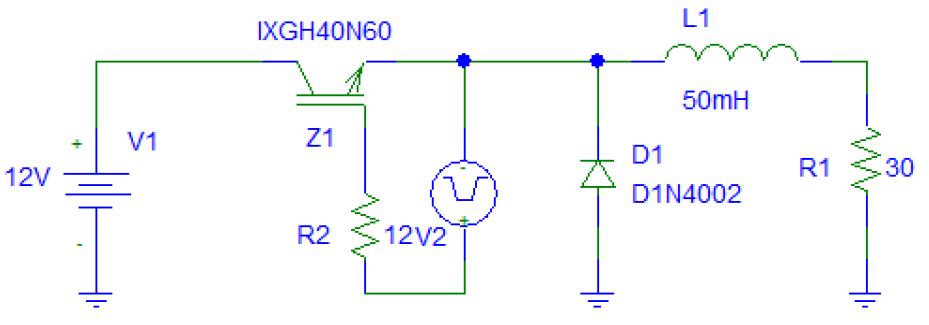
\includegraphics[width = \linewidth]{./pictures/buck.png}}\\
	\cline{1-2}
	DGL
		& $\begin{aligned}
			& i_{L} \cdot R + L\dfrac{di_{L}}{dt} = U_1  & t \in [0; T_{e}]\\
			& i_{L} \cdot R + L\dfrac{di_{L}}{dt} = 0  & t \in [T_{e}; T_{s}]
		\end{aligned}$ & \\
	\cline{1-2}
	Stromverlauf (Lösung der DGL)
		& $i_L = \begin{cases}
					\frac{U_{1}}{R_{1}}+\frac{U_{1}}{R_{1}} \cdot \frac{-1+e^{\frac{-T_{a}}{\tau}}}{1-e^{\frac{-T_{s}}{\tau}}} \cdot e^{\frac{-t}{\tau}} & t \in [0; T_{e}]\\
					\frac{U_{1}}{R_{1}} \cdot \frac{1-e^{\frac{-T_{e}}{\tau}}}{1-e^{\frac{-T_{s}}{\tau}}} \cdot e^{\frac{-(t+T_{e})}{\tau}} & t \in [T_{e}; T_{s}]
			\end{cases}\quad \text{mit} \quad \tau = \frac{L_{1}}{R_{1}}$& \\
	\cline{1-2}
	Ein- und Ausschaltzeiten
		& $\begin{aligned}
			T_{a} &= -\tau \cdot \ln\frac{i_{Lmin}}{i_{Lmax}}\\
			T_{e} &= -\tau \cdot \ln\left(\frac{\zaehlerBuck}{\nennerBuck}\right)\\
			T_{s} &= T_{e} + T_{a}\\
			\tau &= \frac{L_{1}}{R_{1}}
		\end{aligned}$ &\\
	\cline{1-2}
\end{longtabu}
